\chapter{Detailed Design}

\section{Structure Chart}


The proposed maritime surveillance framework is organized as a hierarchical collection of functional modules, each responsible for a specific stage of the surveillance workflow. The structure chart shown in Fig.~\ref{fig:structure} illustrates the modular decomposition of the system, beginning from data acquisition and progressing through vessel detection, tracking, sensor fusion, trajectory prediction, collision risk analysis, and visualization. Such a modular design improves maintainability, scalability, and ease of future system enhancements by allowing individual modules to be developed and upgraded independently.

\begin{figure}[H]
\centering
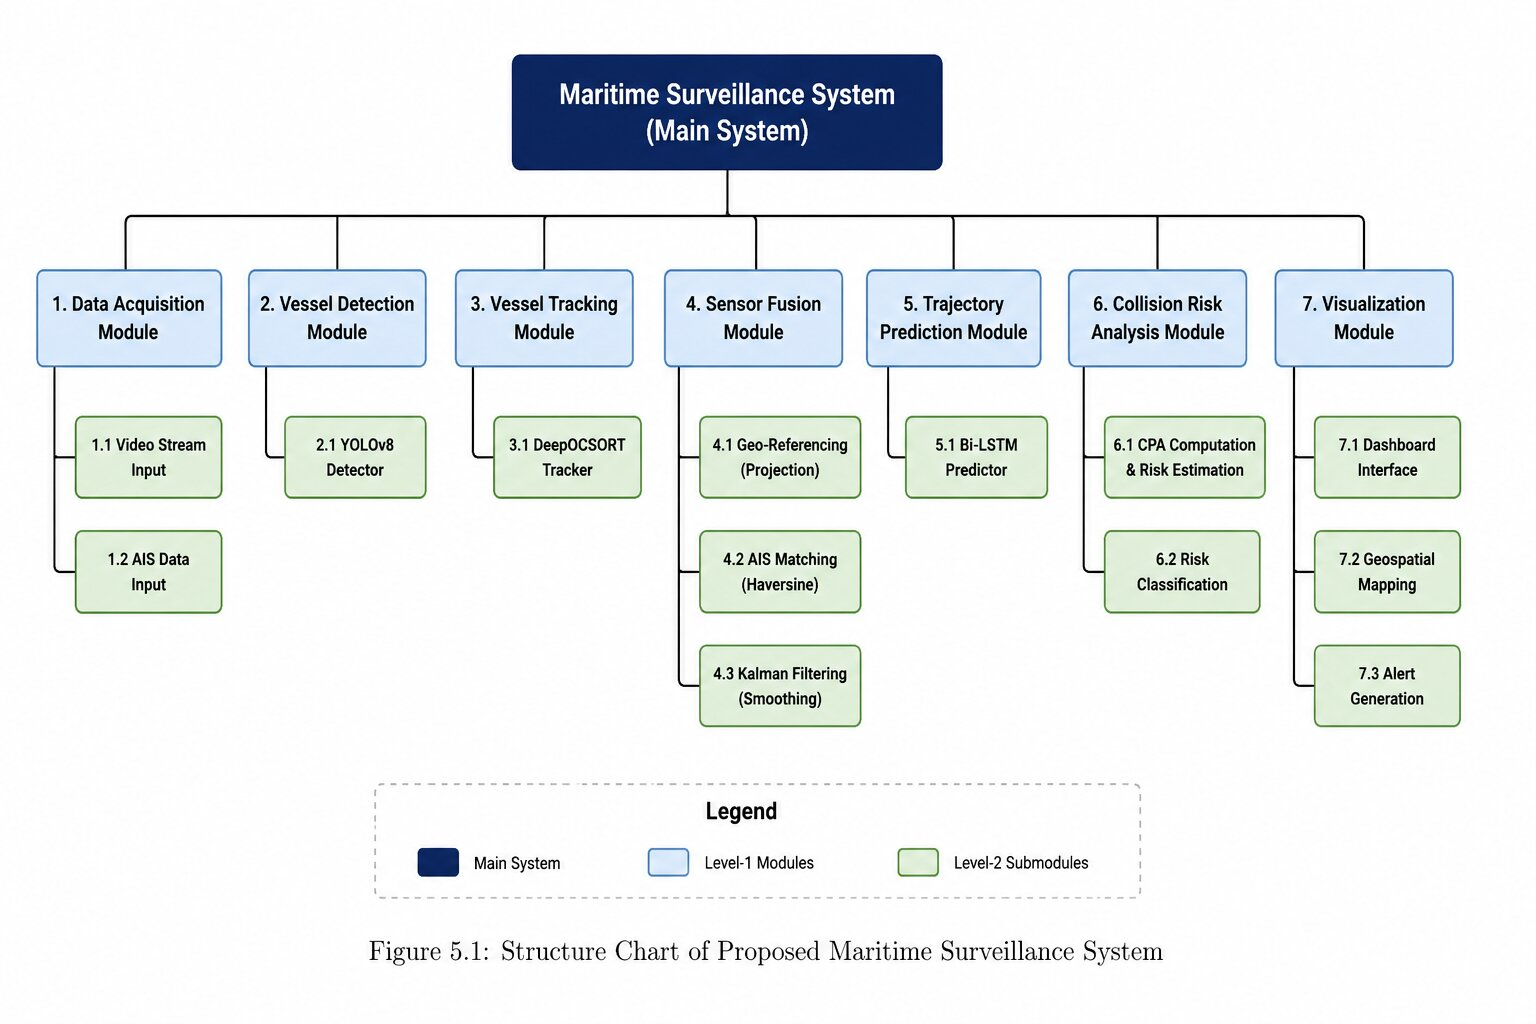
\includegraphics[width=\textwidth]{Chapter5/Figures/structure_chart.jpg}
\caption{Structure Chart of Proposed Maritime Surveillance System}
\label{fig:structure}
\end{figure}

Figure~\ref{fig:structure} illustrates the hierarchical decomposition of the proposed system into functional modules, emphasizing the separation of concerns between data acquisition, perception, fusion, prediction, and visualization components.

\subsection{Design Specifications}
To ensure robust real-time performance, the system is engineered to strict technical parameters. It requires a continuous video feed with a minimum resolution of $1280 \times 720$ pixels, targeting a processing throughput of 30 frames per second. The underlying \gls{yolov8} detection module operates with a confidence threshold of 0.4 and utilizes an \gls{iou} threshold of 0.3 for \gls{nms}, which balances sensitivity against the suppression of false positives. Downstream, the \gls{deepocsort} tracker uses an \gls{osnet} backbone with a cosine similarity metric for appearance-based \gls{reid}. To prevent the proliferation of ghost tracks, the tracker is configured with a maximum track age of 30 frames, a minimum confirmation hit count of 3, and a detection threshold of 0.3.


\begin{table}[H]
\centering
\caption{Design Specifications of the Proposed Maritime Surveillance System}
\label{tab:design_specs}
\begin{tabular}{|l|l|}
\hline
\textbf{Parameter} & \textbf{Specification} \\
\hline
Input Video Resolution & 1280 $\times$ 720 or higher \\
Target Processing Rate & 30 FPS \\
YOLOv8 Confidence Threshold & 0.4 \\
NMS IoU Threshold & 0.3 \\
DeepOCSORT Maximum Age & 30 Frames \\
DeepOCSORT Minimum Hits & 3 Frames \\
Track History Buffer & 90 Frames \\
LSTM Input Sequence Length & 50 Timesteps \\
LSTM Prediction Horizon & 20 Timesteps \\
AIS Matching Radius & 5.5 km \\
Kalman Filter Model & Constant Velocity \\
GPS Conversion Method & Homography / FOV Approximation \\
Hardware Acceleration & NVIDIA CUDA \\
\hline
\end{tabular}
\end{table}



For the predictive modeling phase, the \gls{lstm} module processes a historical sequence of 50 timesteps to forecast the subsequent 20 positions of each vessel. During geospatial mapping, pixel coordinates are mapped to geographic latitude and longitude via a homographic transformation matrix (computed via \texttt{cv2.findHomography} using ground-control points). When such points are unavailable, an \gls{fov} linear approximation serves as a reliable fallback. The derived \gls{gps} positions are smoothed using a per-vessel constant-velocity Kalman filter to mitigate detection jitter. Finally, to ensure physical validity, all forecasted trajectories are validated against a geographic water-area filter. The entire pipeline is implemented in Python, leveraging \gls{pytorch} for deep learning and \gls{opencv} for frame processing, with full support for \gls{nvidia} \gls{cuda} hardware acceleration.

\subsection{Use Case Analysis}
The operational interaction between end-users and the surveillance framework is mapped out in the use case diagram (Figure~\ref{fig:use_case}). It highlights the primary user flows, spanning from raw video acquisition and tracking through to the visualization of predicted trajectories.

\begin{figure}[H]
\centering
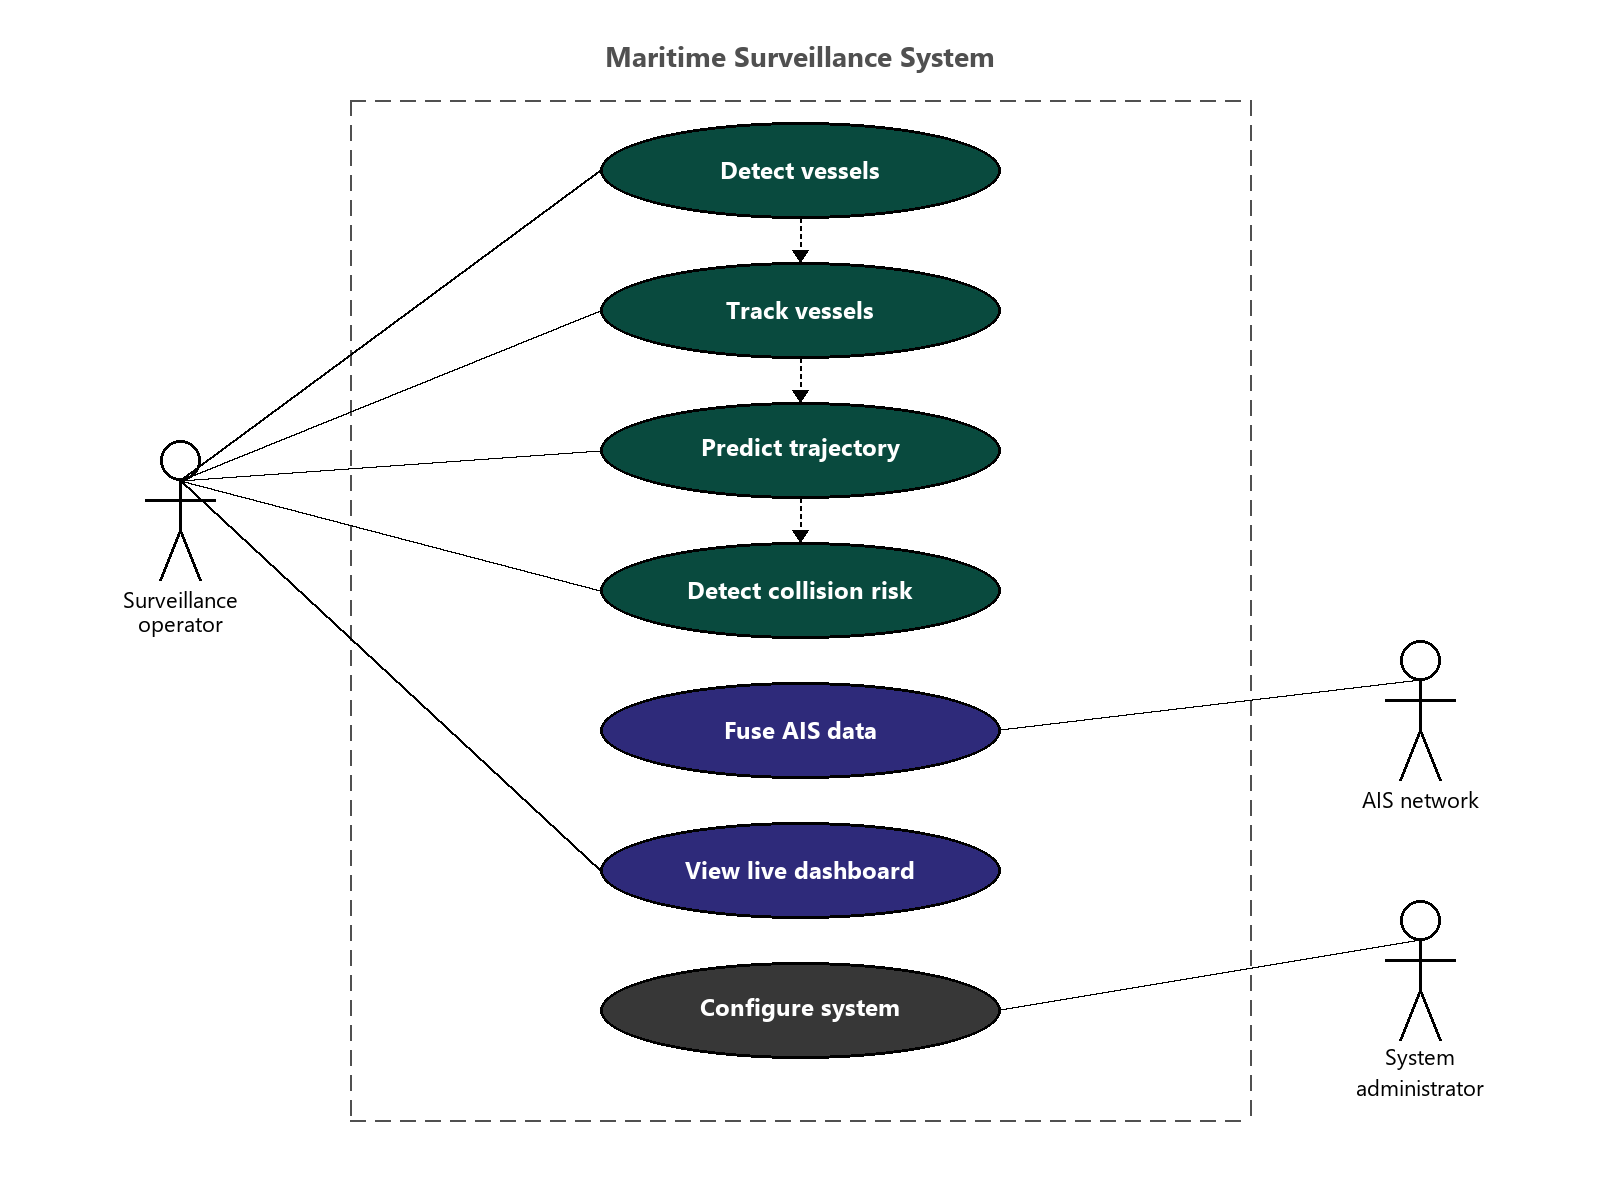
\includegraphics[width=0.95\textwidth]{Chapter3/Figures/fig3_use_case_diagram.png}
\caption{Use Case Diagram of the Maritime Surveillance System}
\label{fig:use_case}
\end{figure}

As shown in Fig.~\ref{fig:use_case}, the operator interacts with the system primarily through the surveillance dashboard, while the internal modules automatically perform vessel detection, tracking, sensor fusion, trajectory prediction, and collision-risk assessment. The use case model highlights the end-to-end functionality available to maritime surveillance personnel.

\subsection{Dataset Analysis and Preprocessing}
The system relies on two specialized datasets: one for fine-tuning the \gls{yolov8} detector, and another for training the \gls{lstm} predictive model. Both were carefully selected based on their environmental diversity, annotation quality, and relevance to maritime scenarios.

For vessel detection, the \textit{Kaggle Ships in Google Earth} dataset (sourced via Roboflow) was utilized. This dataset provides a vast collection of aerial and satellite imagery annotated with \gls{yolo}-formatted bounding boxes. Its diversity in sea states, illumination, and occlusion scenarios makes it highly representative of real-world surveillance environments. The YOLOv8l variant was fine-tuned on this dataset for 70 epochs at a $640 \times 640$ resolution.

Representative samples from the datasets employed for vessel detection and trajectory prediction are shown in Fig.~\ref{fig:dataset_samples}. The figure illustrates the diversity of vessel appearances, scales, viewpoints, and environmental conditions encountered during model development. Such diversity is essential for ensuring the robustness and generalization capability of both the detection and prediction modules.

\begin{figure}[H]
\centering
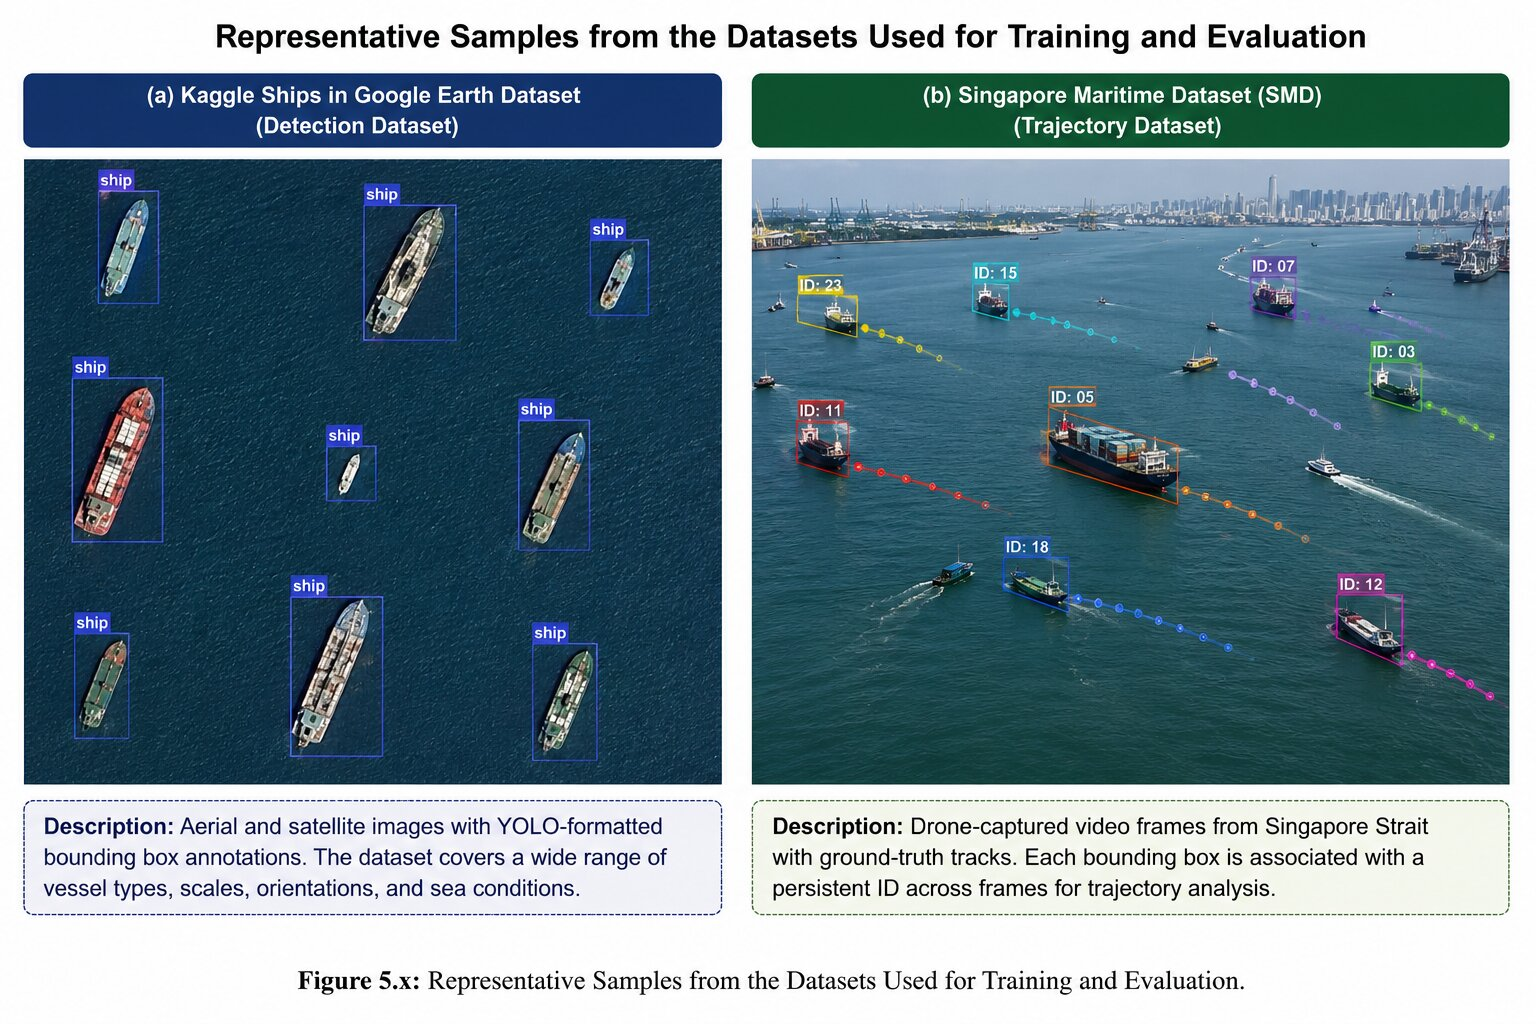
\includegraphics[width=0.95\textwidth]{Chapter5/Figures/dataset_samples.jpg}
\caption{Representative Samples from the Datasets Used for Training and Evaluation}
\label{fig:dataset_samples}
\end{figure}

As shown in Fig.~\ref{fig:dataset_samples}, the vessel detection dataset contains aerial and satellite imagery annotated with vessel bounding boxes, whereas the Singapore Maritime Dataset provides vessel trajectories captured in realistic maritime traffic conditions. Together, these datasets supply complementary information for training the detection and trajectory prediction modules of the proposed system.

Conversely, the \gls{lstm} trajectory model was trained on the \gls{smd}. Captured via drone over the heavily trafficked Singapore Strait, the \gls{smd} provides ground-truth vessel tracks in \texttt{.mat} format. Trajectory centroids are extracted by determining the midpoint of each active bounding box:
\begin{equation}
    x_c = \frac{x_1 + x_2}{2}, \quad y_c = \frac{y_1 + y_2}{2}
    \label{eq:centroid}
\end{equation}
To ensure sufficient historical data for the \gls{lstm} input window, only trajectories spanning a minimum of 50 frames are retained. 

During preprocessing, a sliding window technique (with a stride of 1) divides the raw centroid sequences into a 50-timestep input history and a 20-timestep prediction target. To standardize the inputs, positional coordinates are normalized against the video dimensions:
\begin{equation}
    \hat{x} = \frac{x}{1920}, \quad \hat{y} = \frac{y}{1080}
    \label{eq:normalization}
\end{equation}
Per-frame velocity components are then computed as the first-order differences of these normalized positions:
\begin{equation}
    v_x^{(t)} = \hat{x}^{(t)} - \hat{x}^{(t-1)}, \quad 
    v_y^{(t)} = \hat{y}^{(t)} - \hat{y}^{(t-1)}
   \label{eq:velocity}
\end{equation}
This yields an input feature vector $\mathbf{f}^{(t)} \in \mathbb{R}^4$ at each timestep. The processed dataset is subsequently split 80:20 into training and validation sets using a fixed random seed.

\subsubsection{Evaluation Protocol}

The trajectory prediction model is evaluated using two standard metrics. The prediction performance of the proposed model is assessed using displacement-based evaluation measures that quantify the deviation between predicted and ground-truth vessel trajectories.

The \textit{Average Displacement Error} (\gls{ade}) computes the mean Euclidean distance between the predicted and actual positions across all forecasted timesteps:
\begin{equation}
    \text{ADE} = \frac{1}{K} \sum_{k=1}^{K} \sqrt{(\hat{x}_k - x_k)^2 + (\hat{y}_k - y_k)^2}
    \label{eq:LSTM1}
\end{equation}
Meanwhile, the \textit{Final Displacement Error} (\gls{fde}) assesses accuracy exclusively at the final predicted timestep:
\begin{equation}
    \text{FDE} = \sqrt{(\hat{x}_K - x_K)^2 + (\hat{y}_K - y_K)^2}
    \label{eq:LSTM2}
\end{equation}
These metrics are compared against a kinematic linear baseline to quantify the percentage improvement provided by the \gls{lstm}.

\subsection{Algorithmic Selection}


The selection of the core algorithms—\gls{yolov8} for detection, \gls{deepocsort} for tracking, and \gls{lstm} for prediction—was driven by comparative benchmarking against alternative architectures. Table~\ref{tab:algorithm_comparison} summarizes the selected algorithms and the principal alternatives that were evaluated during the design phase.


\begin{table}[H]
\centering
\caption{Algorithm Selection Comparison}
\label{tab:algorithm_comparison}
\begin{tabular}{|l|l|l|}
\hline
\textbf{Task} & \textbf{Selected Algorithm} & \textbf{Alternative Methods} \\
\hline
Vessel Detection & YOLOv8 & YOLOv5, Faster R-CNN \\
Multi-Object Tracking & DeepOCSORT & SORT, DeepSORT \\
Trajectory Prediction & Bi-LSTM & GRU, Kalman Filter \\
\hline
\end{tabular}
\end{table}

As shown in Table~\ref{tab:algorithm_comparison}, the chosen algorithms provide the best balance between accuracy, robustness, and real-time performance for maritime surveillance applications. Each algorithm was selected based on its ability to address specific challenges associated with vessel detection, identity preservation, and long-horizon trajectory prediction.

\gls{yolov8} outperformed other YOLO variants primarily due to its anchor-free detection head and decoupled classification branches. In maritime environments, the aspect ratios of vessels vary wildly depending on the camera angle; an anchor-free design eliminates the need to predefine these ratios. Furthermore, its optimized feature pyramid network excels at multi-scale aggregation, allowing the system to detect massive cargo ships and tiny distant fishing boats simultaneously.

For tracking, motion-only algorithms like \gls{sort} were rejected because they rely solely on spatial overlap (\gls{iou}). In busy ports where vessels frequently cross paths or become occluded, this leads to severe identity switching. \gls{deepocsort} solves this by incorporating an \gls{osnet} appearance descriptor, meaning the tracker remembers what a ship *looks like* as well as where it was heading. 

Finally, \gls{lstm} networks were chosen over Kalman filters and \glspl{gru} for trajectory prediction. While Kalman filters are computationally lightweight, they assume linear, constant-velocity motion, which fails to capture the non-linear maneuvering of real ships. Although \glspl{gru} offer a lighter neural alternative, the dedicated gating mechanisms of an \gls{lstm}—specifically its separate input, forget, and output gates—proved vastly superior at retaining the long-range temporal dependencies required to predict complex nautical turns. 

The rationale behind the selection of the core algorithms used in the proposed system is illustrated in Fig.~\ref{fig:algorithm_selection}. The figure compares the selected methods against commonly used alternatives and highlights the primary factors that influenced their adoption.

\begin{figure}[H]
\centering
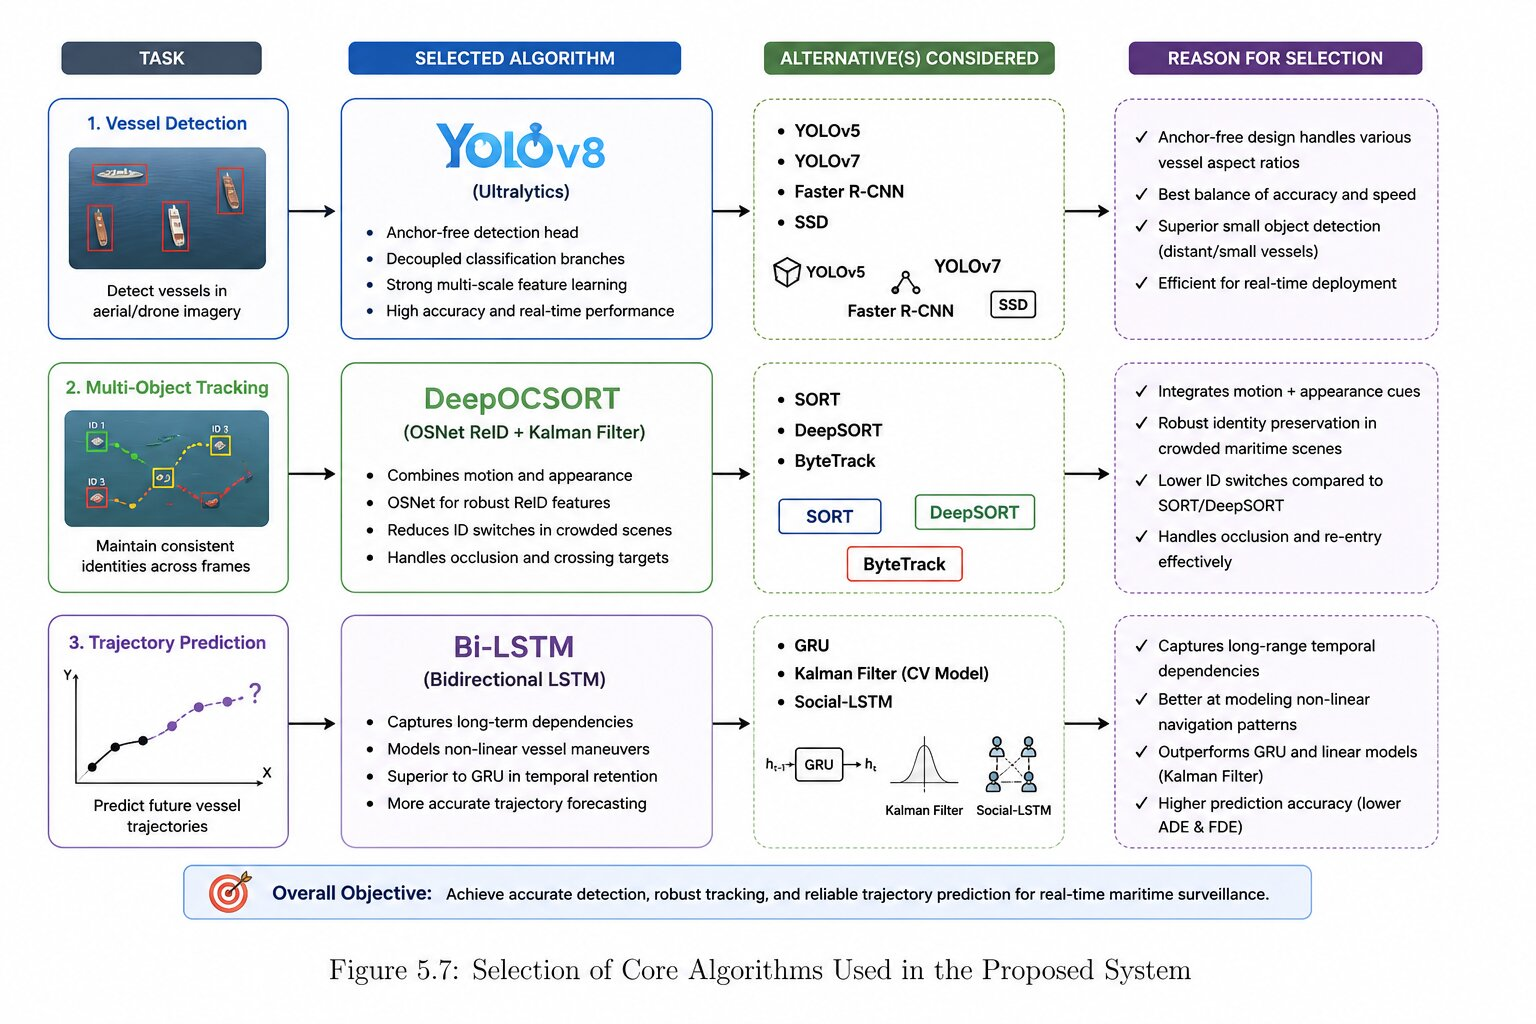
\includegraphics[width=0.95\textwidth]{Chapter5/Figures/algorithm_selection.jpg}
\caption{Selection of Core Algorithms Used in the Proposed System}
\label{fig:algorithm_selection}
\end{figure}

Figure~\ref{fig:algorithm_selection} demonstrates that YOLOv8 was selected because of its anchor-free architecture and strong real-time detection capability, while DeepOCSORT was preferred for its ability to combine motion and appearance information for robust vessel identity tracking. Similarly, the Bi-directional LSTM model was adopted due to its capability to capture long-term temporal dependencies and accurately model non-linear vessel movement patterns, resulting in improved trajectory prediction performance compared to conventional approaches.



\subsection{Data Fusion and Processing Pipeline}

The proposed maritime surveillance framework follows a multi-stage processing pipeline that integrates computer vision, sensor fusion, trajectory prediction, and visualization components into a unified operational workflow. Raw video streams and AIS messages are processed concurrently, allowing the system to combine visual observations with navigational telemetry. The end-to-end processing pipeline, illustrated in Fig.~\ref{fig:pipeline}, demonstrates how information flows through successive stages of detection, tracking, coordinate transformation, data fusion, trajectory prediction, and decision support.

\begin{figure}[H]
\centering
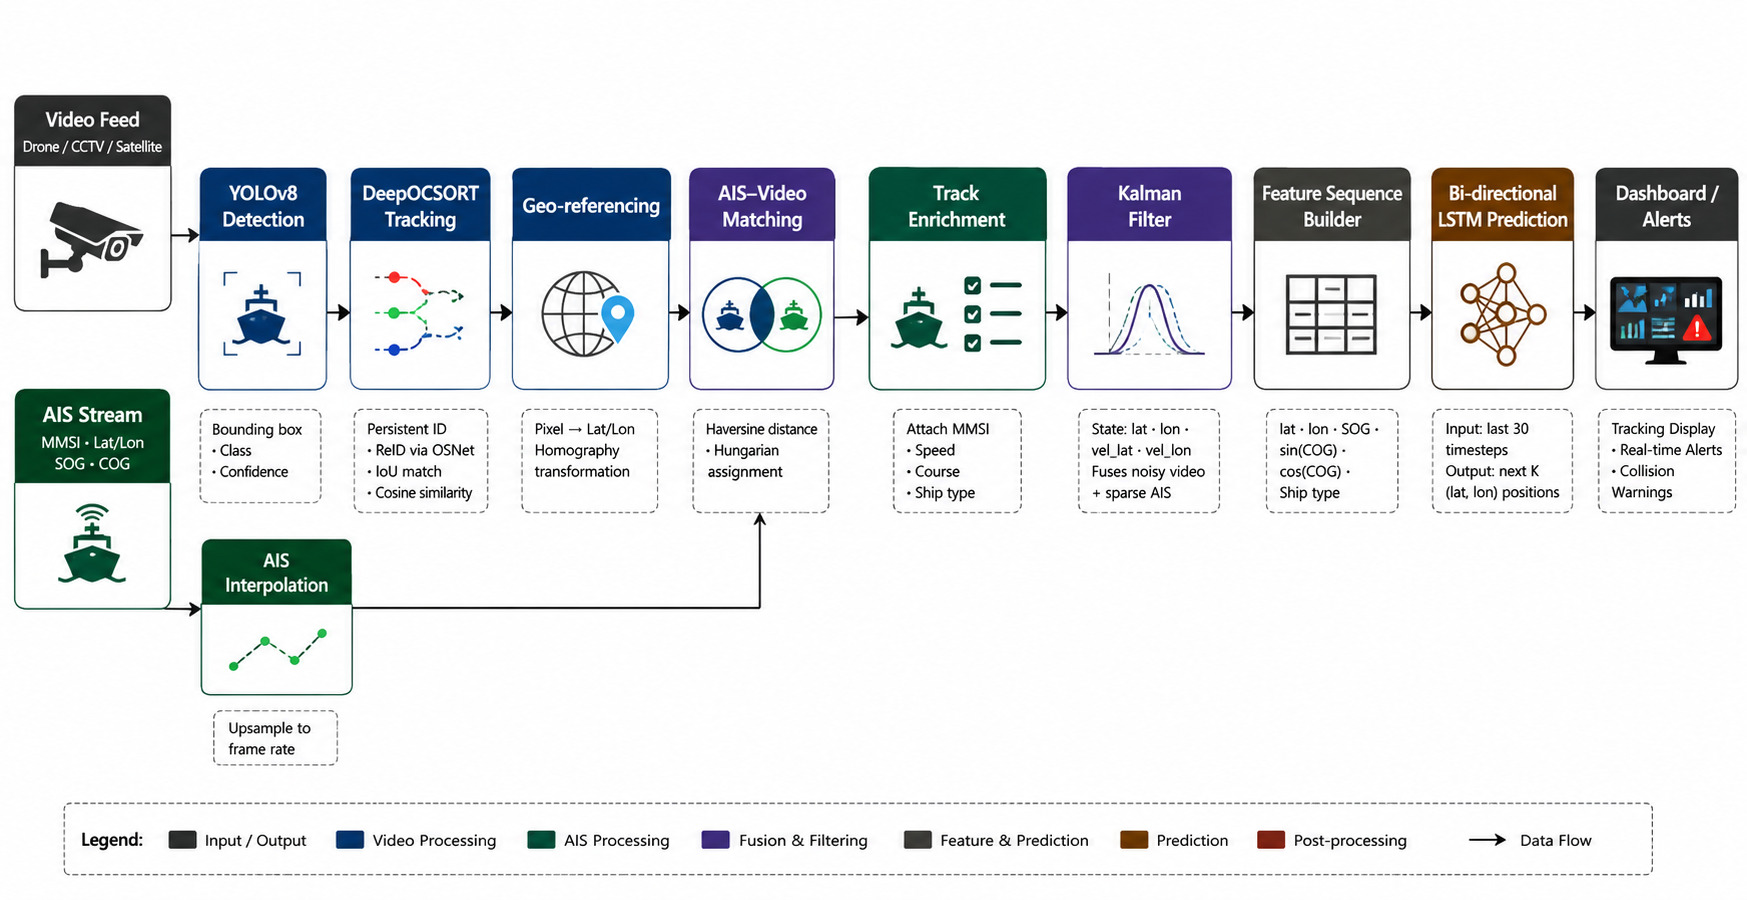
\includegraphics[width=0.85\textwidth]{Chapter3/Figures/process_pipeline.jpeg}
\caption{End-to-End Processing Pipeline of Proposed Maritime Surveillance System}
\label{fig:pipeline}
\end{figure}

As shown in Fig.~\ref{fig:pipeline}, the workflow begins with video ingestion and AIS acquisition. Video frames are processed by the YOLOv8 detector to identify vessel instances, while the DeepOCSORT tracker maintains persistent identities across consecutive frames. The tracked vessel positions are subsequently transformed from image coordinates into geographic coordinates before being associated with AIS observations. The fused vessel states are then supplied to the trajectory prediction module, which forecasts future vessel movement and supports downstream collision-risk assessment and maritime situational awareness.


The core of this pipeline is the sensor fusion strategy, which leverages the complementary strengths of both data sources. Video tracking provides rapid, frame-by-frame updates but suffers from pixel-projection noise. Conversely, \gls{ais} data offers highly precise \gls{gps} coordinates and rich metadata (such as \gls{mmsi} and vessel name) but updates sparsely. To fuse them, the system employs a nearest-neighbor association using the Haversine great-circle distance. 

When a vessel is detected on camera, its pixel position is converted to a geographic coordinate, smoothed via a Kalman filter, and compared against the live \gls{ais} registry. If an \gls{ais} record exists within a 5.5\,km radius, the visual track is enriched with the \gls{ais} metadata. If no match is found, the vessel is flagged as a \textit{dark vessel}—a potentially non-cooperative craft operating without an active transponder.

This fusion strategy significantly improves the reliability of vessel monitoring by combining the high temporal resolution of video observations with the positional accuracy and contextual metadata provided by AIS transmissions. Furthermore, the ability to identify unmatched visual detections enables the system to detect potentially non-cooperative or suspicious vessels that may otherwise remain absent from conventional AIS-based monitoring systems.


\section{Module Description}

\subsection{System Execution Flow}

The operational workflow followed by the proposed maritime surveillance framework is represented by the flowchart shown in Fig.~\ref{fig:flowchart}. The flowchart illustrates the logical sequence of operations performed by the system, beginning with data acquisition and progressing through vessel detection, tracking, AIS fusion, trajectory prediction, and collision analysis.

\begin{figure}[H]
\centering
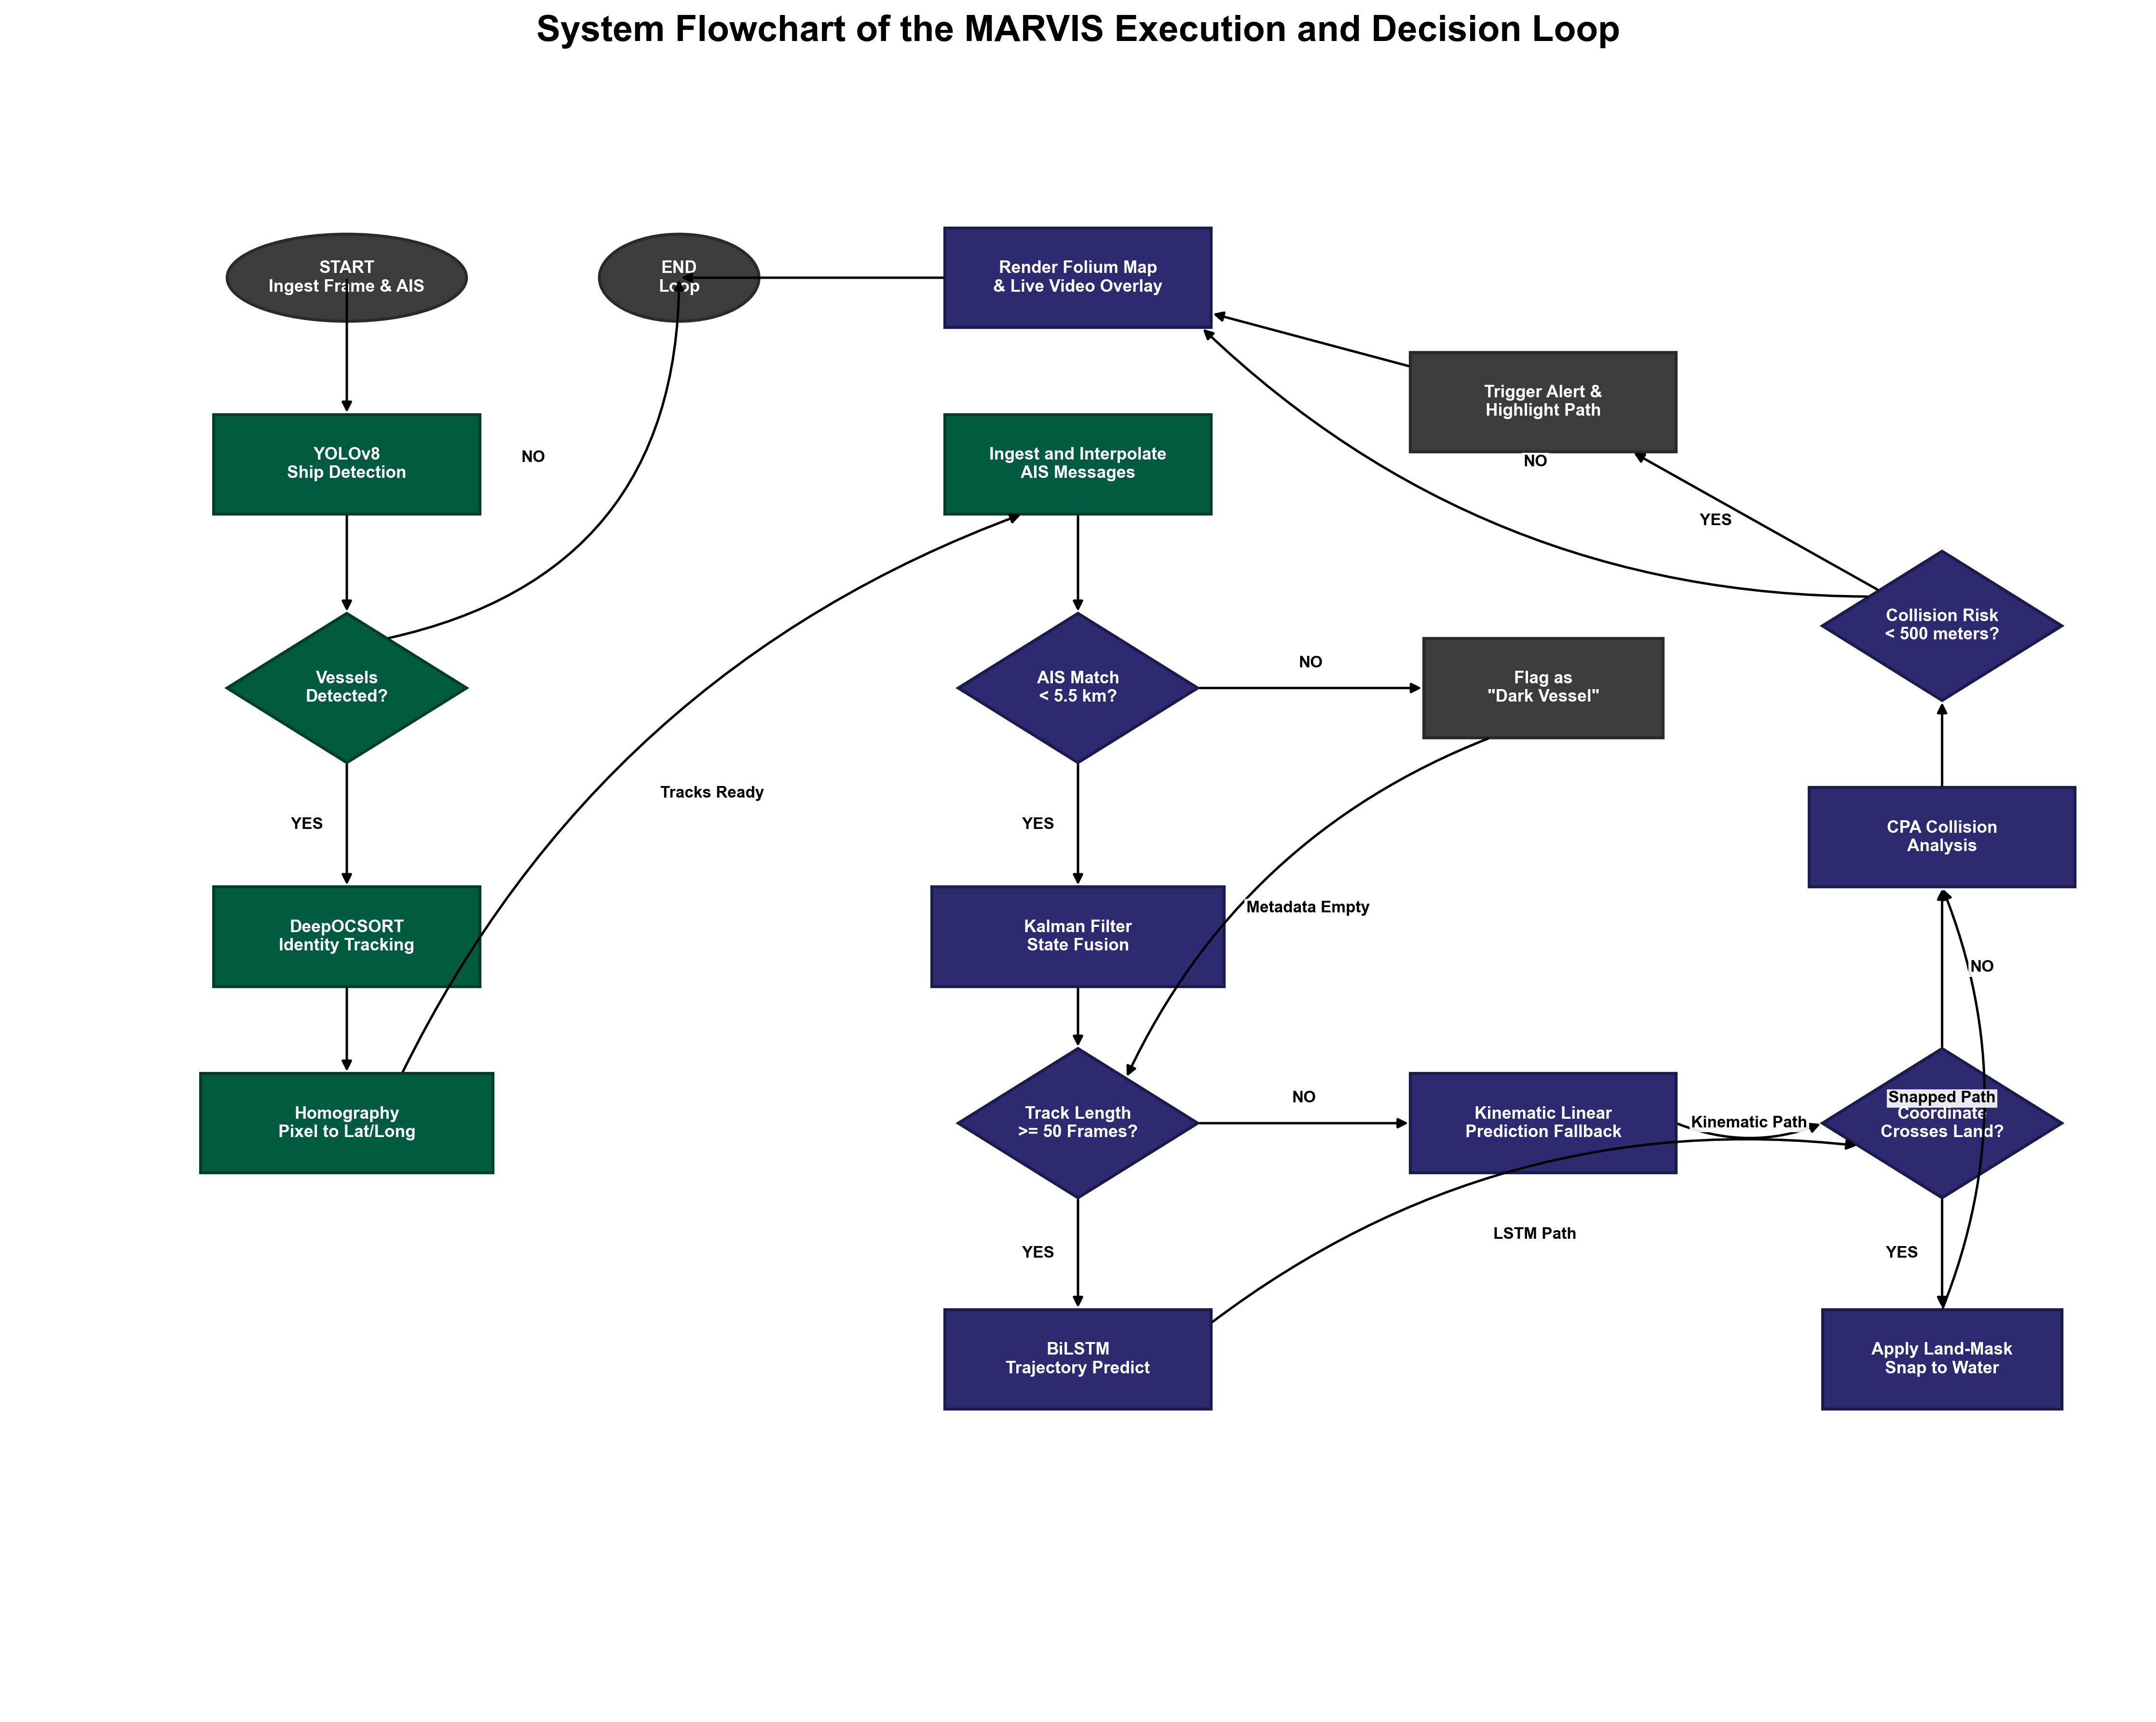
\includegraphics[width=0.9\textwidth]{Chapter5/Figures/pipeline_flowchart.png}
\caption{System Execution Flowchart of the Proposed Maritime Surveillance Framework}
\label{fig:flowchart}
\end{figure}

As shown in Fig.~\ref{fig:flowchart}, the system continuously processes incoming video frames and AIS messages while evaluating a series of decision points. These include vessel detection validation, AIS association, trajectory prediction eligibility, collision-risk assessment, and alert generation. Such a structured execution workflow ensures that the surveillance pipeline operates reliably under real-time conditions.

\subsection{System Interaction Sequence}

The interaction between the major software components of the proposed system is illustrated using the sequence diagram shown in Fig.~\ref{fig:sequence}. The diagram captures the chronological exchange of information between data acquisition modules, tracking components, sensor fusion services, prediction models, and visualization interfaces.

\begin{figure}[!htbp]
\centering
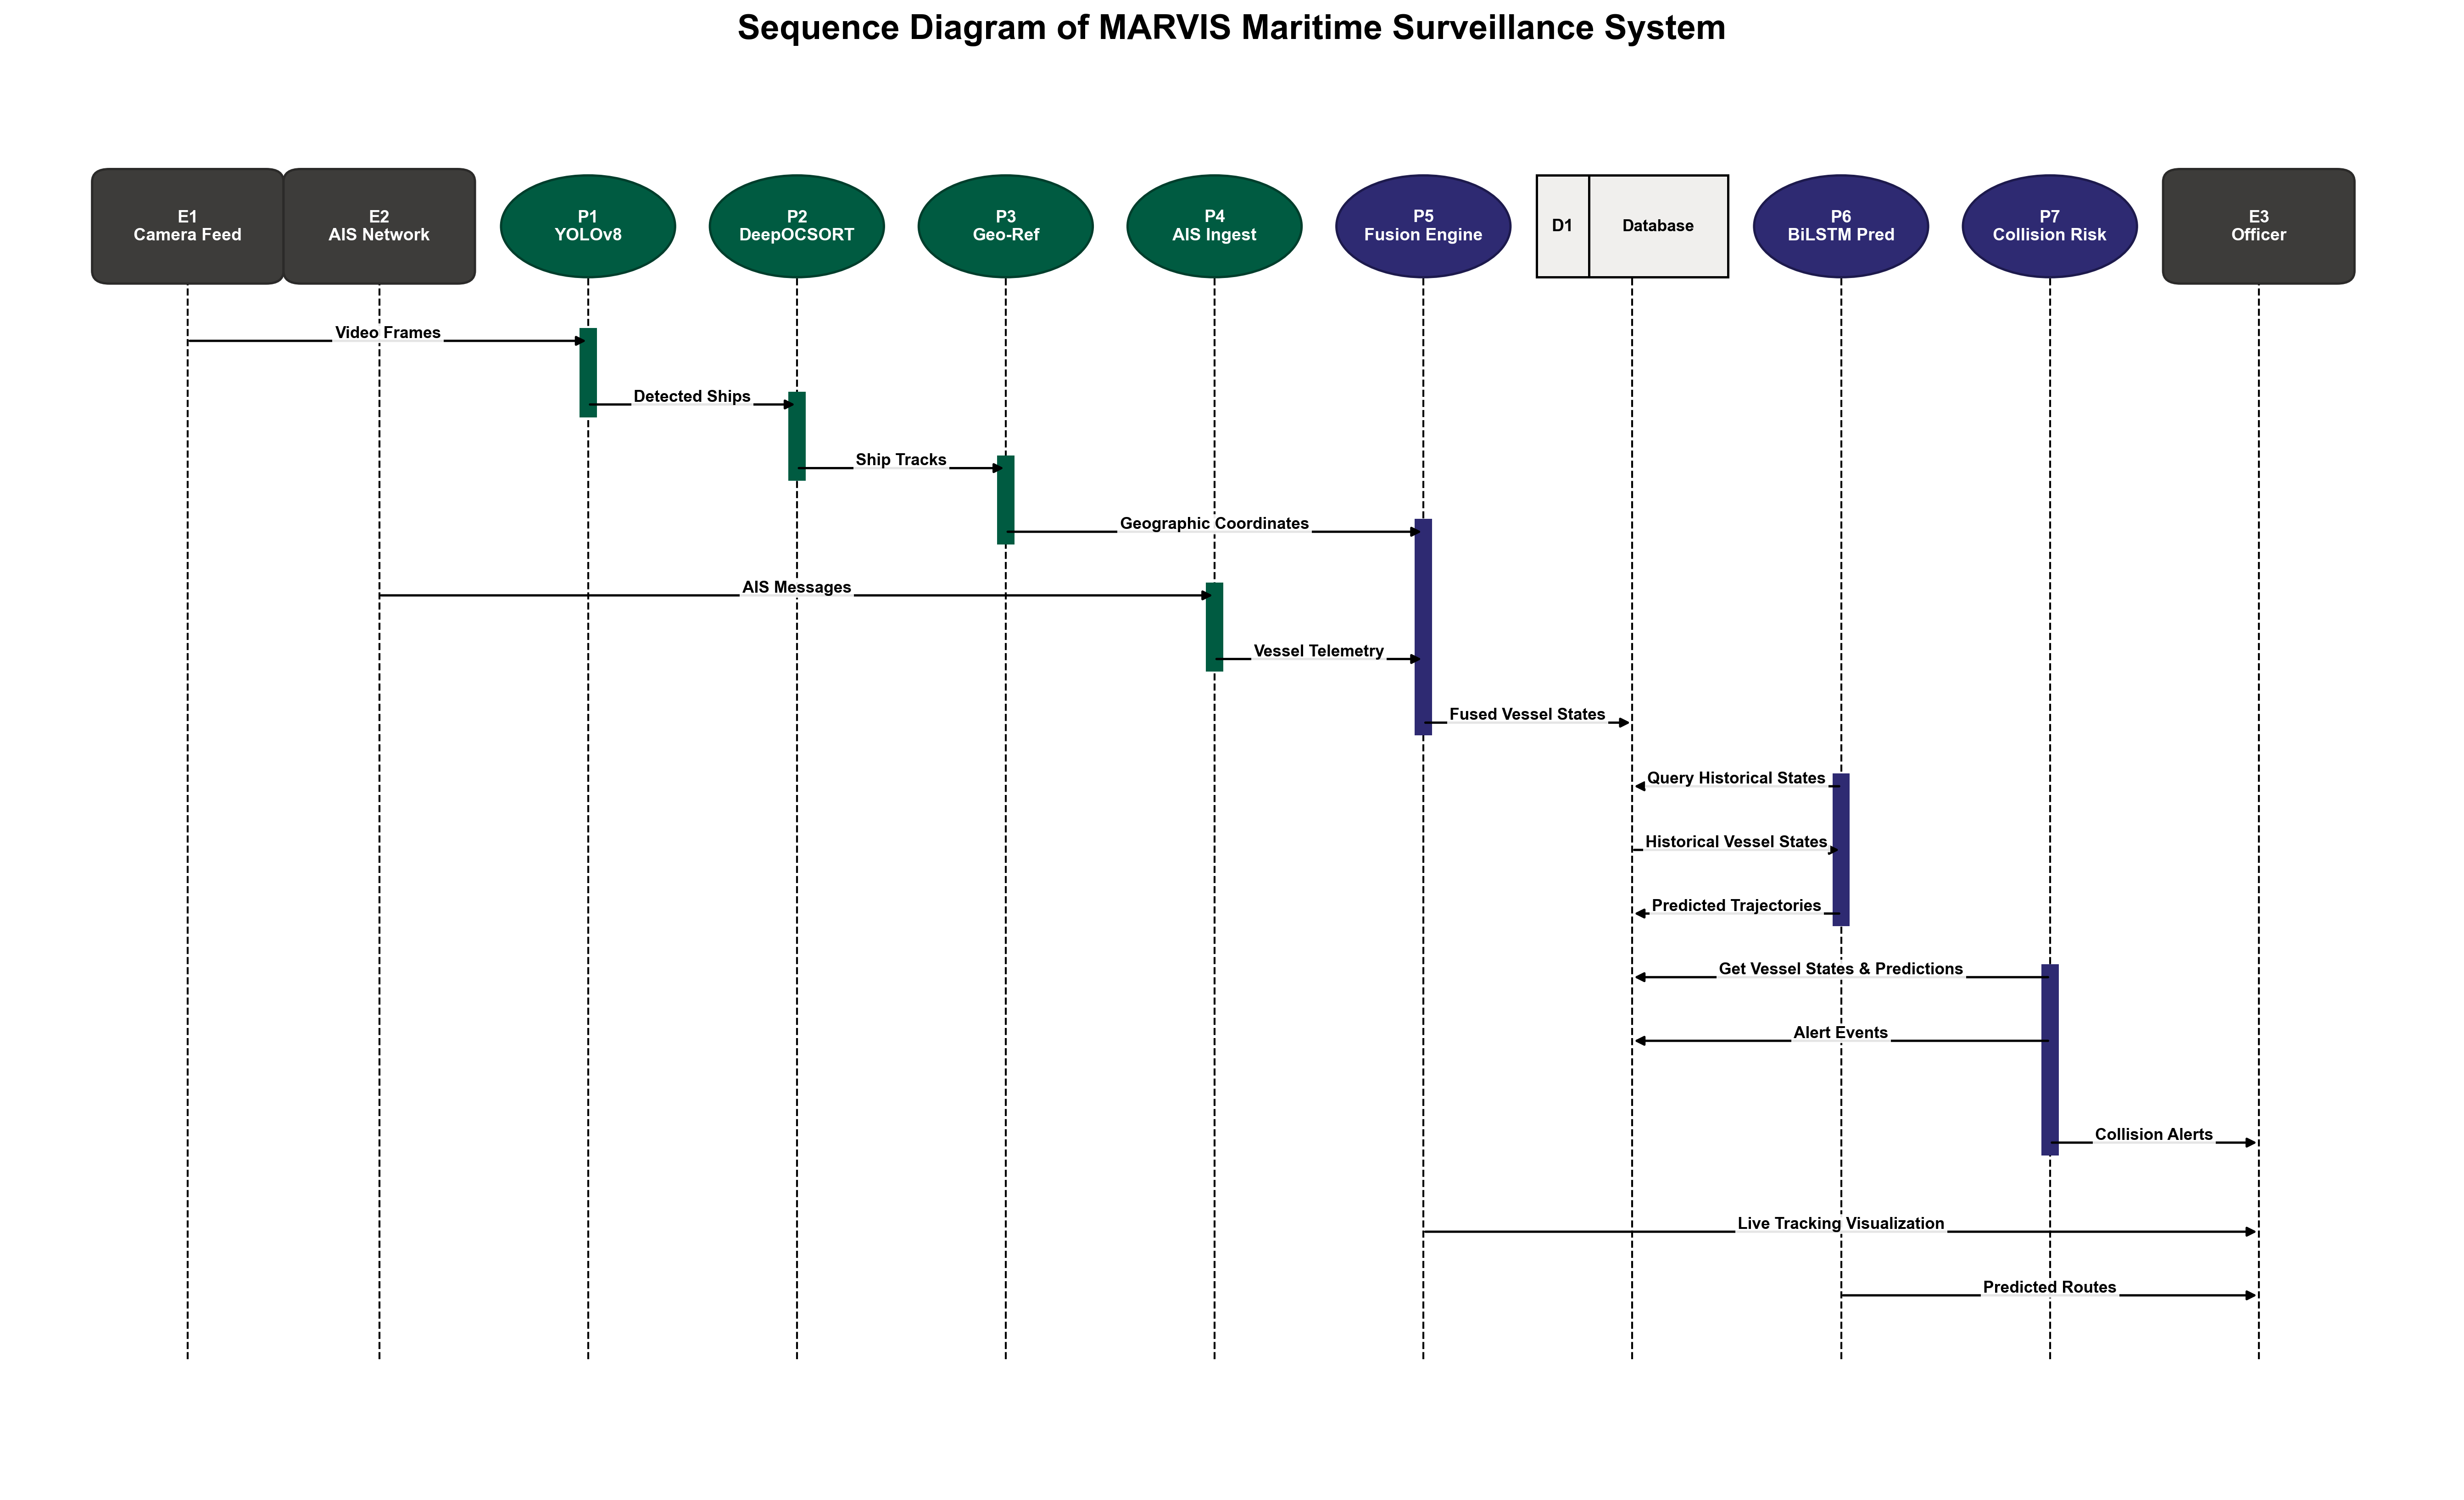
\includegraphics[width=\textwidth]{Chapter5/Figures/sequence_diagram.png}
\caption{Sequence Diagram of the Proposed Maritime Surveillance System}
\label{fig:sequence}
\end{figure}

Figure~\ref{fig:sequence} shows that video frames and AIS messages are processed concurrently before being fused into a unified vessel representation. The fused vessel state is then supplied to the trajectory prediction module, which generates future vessel positions for collision-risk assessment and dashboard visualization. The sequence diagram demonstrates the temporal coordination required among all modules to achieve real-time maritime surveillance.

\subsection{Functional Module Description}
Rather than treating the system as a monolith, the architecture is divided into specialized, interconnected modules that handle specific operational tasks:

\subsubsection{Data Acquisition Module}
The \textbf{Data Acquisition Modules} manage the ingestion of raw information. The \gls{ais} receiver extracts identifiers and navigational telemetry, while the video processing module handles frame extraction and normalization for downstream computer vision tasks. 

\subsubsection{Vision and Tracking Module}
Following ingestion, the \textbf{Vision and Tracking Modules} take over. \gls{yolov8} generates bounding boxes around all visible ships, and \gls{deepocsort} assigns persistent identities to these detections, ensuring continuity even if a vessel briefly passes behind an obstruction.

\subsubsection{Transformation and Fusion Module}
The data is then contextualized by the \textbf{Transformation and Fusion Modules}. Image-space coordinates are mathematically projected into real-world geographic coordinates. This allows the data fusion engine to pair the visual observations with the corresponding \gls{ais} telemetry, resulting in a highly reliable, metadata-enriched vessel track.

\subsubsection{Analytical and Visualization Module}
Finally, the \textbf{Analytical Modules} generate actionable intelligence. The trajectory predictor uses a \gls{bilstm} network to forecast future movements based on historical patterns, while the collision detection system analyzes these forecasts to flag potential intersecting paths. All of this information is synthesized by the visualization module, which renders the bounding boxes, predicted paths, and alert notifications onto an intuitive operator dashboard.

\section{Summary}

This chapter detailed the foundational design and methodology of the proposed maritime surveillance system. Operational parameters were established and justified across the entire pipeline, from the confidence thresholds of the \gls{yolov8} detector to the memory buffer configurations of the \gls{deepocsort} tracker. The selection of these specific architectures was defended through comparative analysis against alternatives like \gls{sort} and \glspl{gru}, emphasizing the need for robust performance under challenging, real-world maritime conditions. 

Furthermore, a rigorous mathematical framework was established to govern the pixel-to-coordinate transformations, Haversine fusion metrics, and\gls{lstm} error calculations (Equations~\ref{eq:centroid}--\ref{eq:LSTM2}). By routing the data through a carefully structured sequence of functional modules—from raw video ingestion through to collision analysis and dashboard rendering—the system provides a cohesive, scalable solution for intelligent vessel monitoring.